\chapter{Results and Discussion}
This chapter presents the results of training the Explainable Boosting Machine (EBM) on the extracted linguistic
features from the I-JAS corpus. The section begins with an overview of the model's performance, followed by an
analysis of feature importance and concludes with a discussion of the results in light of previous findings and
methodological considerations.


\section{Model Performance}
%*Discuss f1, accuracy, precision
%*share confusion matrix
%*discuss small sample size for N1 group which likely affected the classification
%*could not achieve better than 50\% accuracy, probably due to the 5 groups and overlap between some proficiency
%levels. Still better performance than the 20\% random guess baseline....

The EBM was trained using the full set of extracted features on a five-class classification task corresponding to
the five JLPT proficiency levels (N5-N1). Interactions were set to 0 to allow for clear interpretation of the
feature importances. The model was
evaluated using 5 fold cross validation,
with over sampling to balance the minority classes (N1 and N5). The results, aggregated across all cross validation
folds, are summarized
in Table~
\ref{tab:trainingResults}.


\begin{table}[h!]
    \centering
    \begin{tabular}{lcccc}
        \hline \textbf{Class} & \textbf{Precision} & \textbf{Recall} & \textbf{f1-score} & \textbf{Support} \\ \hline
        N5    &   0.45   &   0.51   &   0.48   &    735\\
          N4    &   0.43   &   0.39   &   0.41   &   1431\\
          N3    &   0.38   &   0.34   &   0.36  &    1342\\
          N2  &     0.34   &   0.38  &    0.36   &    816\\
          N1    &   0.15   &   0.19   &   0.17    &   224\\ \hline
        accuracy &   -    &      -    &     0.38  &    4548\\
   macro avg  &     0.35   &   0.36  &    0.35   &   4548\\
weighted avg  &     0.39  &    0.38    &  0.38   &   4548\\ \hline
    \end{tabular}
    \caption[Overall Classification Report (All Folds Combined)]{Overall Classification Report (All Folds Combined)}
    \label{tab:trainingResults}
\end{table}

The model achieved an overall accuracy of 38\%, demonstrating some capacity to distinguish between proficiency
levels.
While the overall performance did not exceed 50\%, it represents a significant improvement over a random guess
baseline of 20\% for a five-class classification problem. The F1-scores, which provide a harmonic mean of precision
and recall ranged from .15 for N1 and .45 for N5 (Table~\ref{tab:trainingResults}).

Notably, classification performance declined as proficiency increased, with the N1 group showing the weakest
performance across all metrics (precision = 0.15, recall=0.19, f1=0.17). This is likely attributable in part to the
small sample size of N1 texts in the corpus, as well as the overlap between the proficiency levels.

Performance was highest for the N5 and N4 levels, which may reflect the chosen features may be more robust against
distinguishing the lower proficiency and intermediate levels. In contrast, the model struggled to differentiate
adjacent intermediate levels N3-N2, which suggests a need for more sensitive or diversified features as shown in the
confusion matrix in Figure~\ref{fig:conMA}.

\begin{figure}[h!]
           \centering
           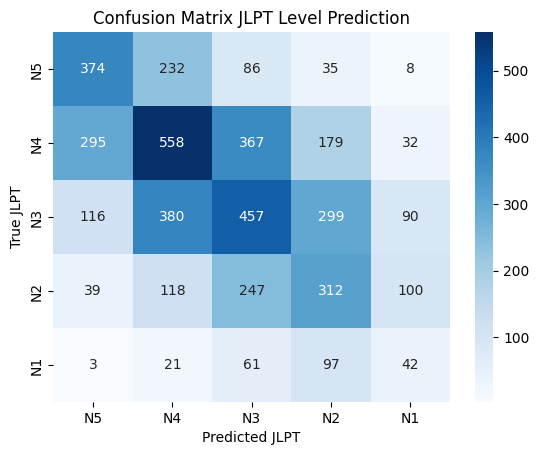
\includegraphics[scale=.4]{img/confusionMatrix}
           \caption[Confusion Matrix for JLPT Level Prediction]{Confusion Matrix for JLPT Level Prediction}
           \label{fig:conMA}
\end{figure}

A common mis-classification was a substantial number of true N3 instances were misclassified as N4(380) or N2 (299).
Similarly, N2 texts were frequently predicted as N3(245) or N1 (107), and N1 texts were often misclassified as N2(
98) or N3(62). This suggests that the model frequently confused text belonging to adjacent proficiency levels,
indicating a high overlap between the proficiency levels. This was confirmed when

This overlap was further supported when aggregating the proficiency levels into broader 3 groups - Beginner (N5+N4),
Intermediate (N3+N2), and
Advanced (N1).
Classification performance for these three groups improved significantly, achieving an overall F1-score of .54. This
substantial increase from .38 F1-score for the five-lcass problem further corroborates the hypothesis that the
continuous nature of adjacent JLPT levels present a significant challenge for fine-grained classification.

\section{Feature Importance Analysis}
\begin{figure}[h!]
    \centering
    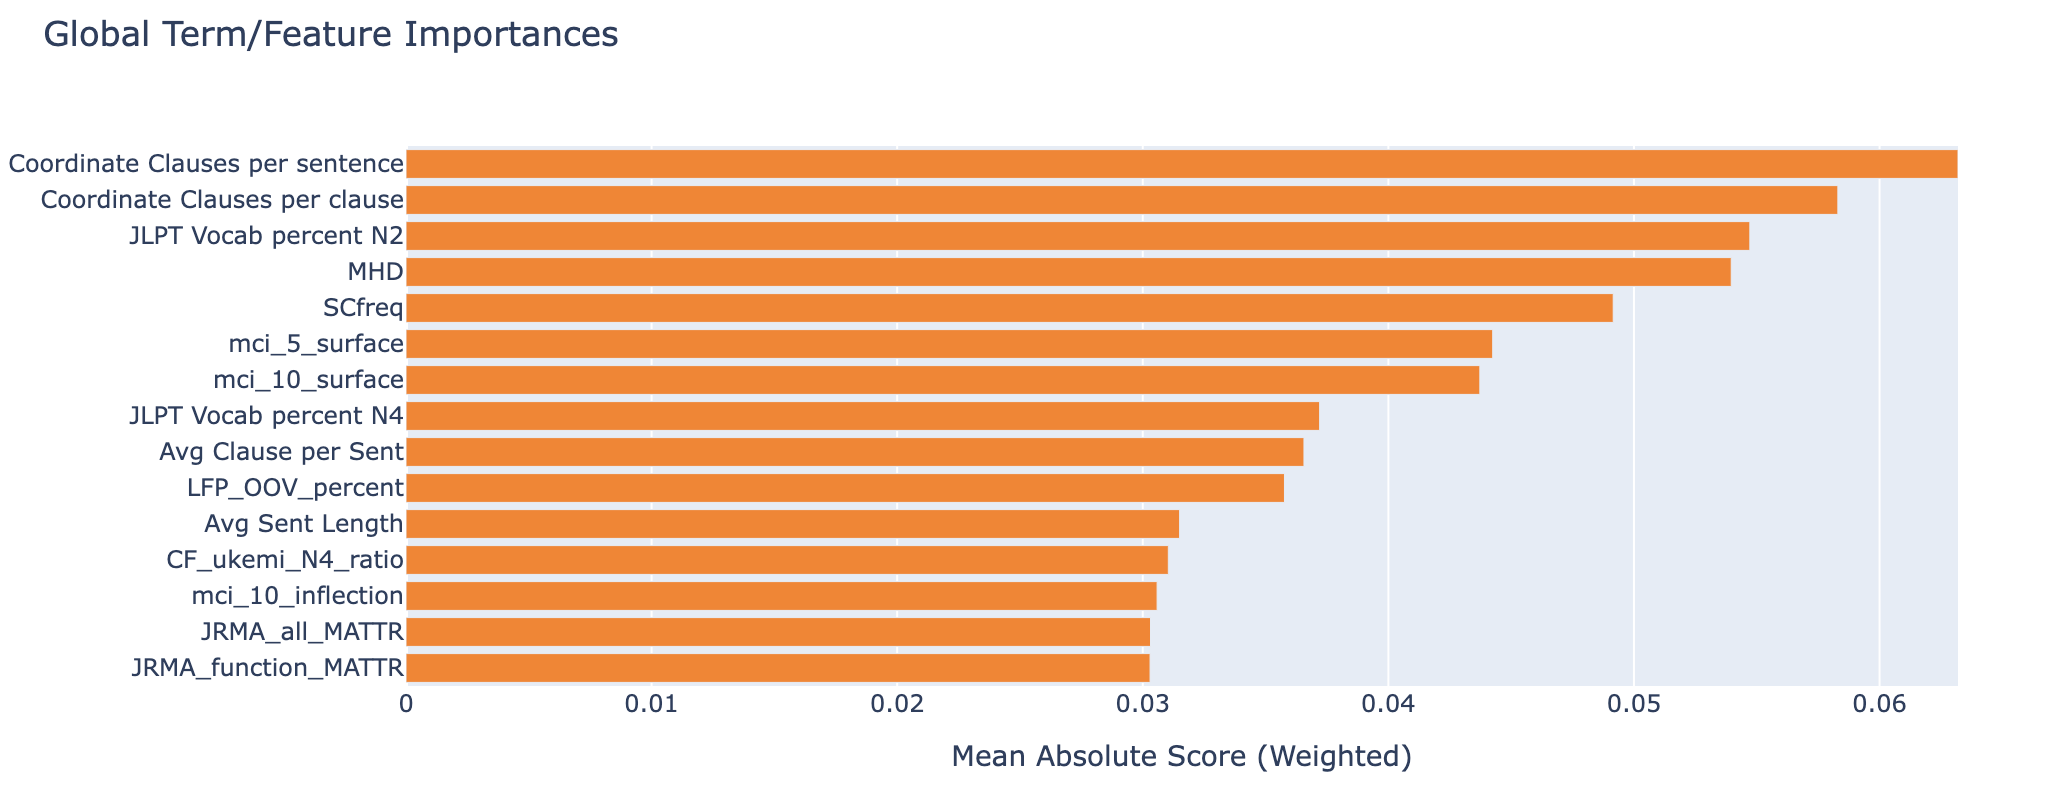
\includegraphics[scale=.4]{img/feature_importance}
    \caption[Feature Importance Chart]{ Feature Importance Chart: Top-ranked features contributing to the classifcation of JLPT proficency levels, based on thier additive contribution scores from the EBM model.}
    \label{fig:featureimportance}
\end{figure}


The feature importance results from the final EBM model are shown in Figure~\ref{fig:featureimportance}. Overall, a
diverse range of linguistic features contributed to classification accuracy, though complexity measures were most
prominent among the top-ranked features. A diverse variety of complexity
measures from Syntactic to lexical, and morphological contributed to the classification indicating that indeed, a
wide variety of features are needed to classify learner texts.

The top two features were coordinate clauses per sentence and coordinate clauses per clause, both measures of
syntactic complexity. These features suggest that the frequency of coordination structures is a strong
differentiator across proficiency levels, potentially a reflection of developmental gains in syntactic elaboration. This
also makes sense as this feature as also found in the previous section to discriminate between adjacent levels in
the low to mid-proficiency ranges while also being used more frequently at the higher proficiency levels. The class
separation can be seen in Figure~\ref{EBMccPerSent}, where N5 shows a strong positive score when the CC per sentence
measure is lower than .25, whereas a measure above 1 is shown to be associated with N1, and the higher proficiency
levels. In other words, a lower score indicates lower
proficiency.

\begin{figure}[h!]
    \centering
    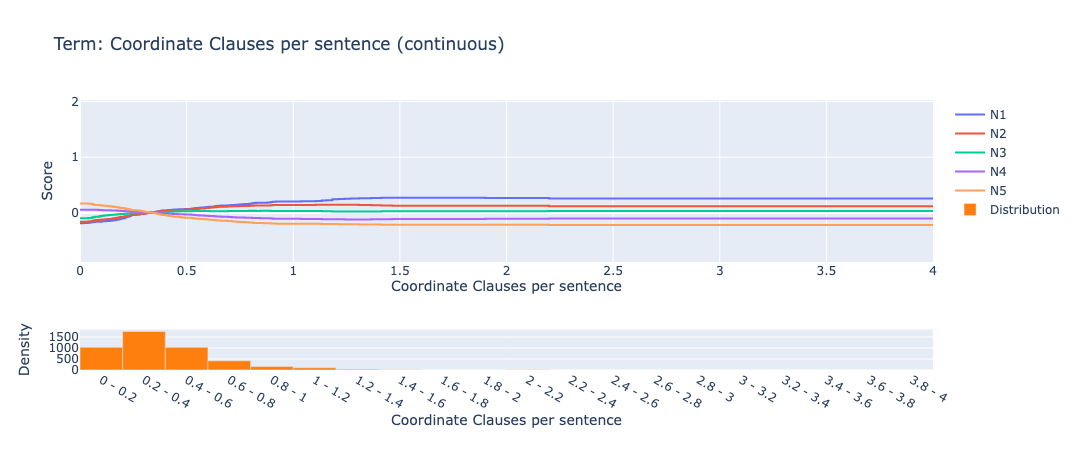
\includegraphics[scale=.4]{img/EBM/EBMccPerSent}
    \caption[Contribution of Coordinate Clauses per Sentence]{This chart represents how the feature of Coordinate clauses per sentence conributes to the prediction of each proficiency level}
    \label{fig:EBMccPerSent}
\end{figure}


The third-ranked feature, ratio of words from JLPT N2 list to token ratio (Lexical Frequency Profile), highlights
lexical sophistication as another important dimension. A higher proportion of N2-level vocabulary appears to
correlate with higher proficiency levels, aligning with expectations from previous lexical profiling studies
\citep{Laufer1995}. This feature was also found to distinguish reliably between the higher proficency levels. As can
be seen in Figure~\ref{fig:EBMjlptN2}, there is spread between the N1 and N2 lines while the other proficiency
levels overlap. Meaning this measure distinguished
the N1 and N2 levels from the begining levels.

\begin{figure}[h!]
    \centering
    \includegraphics[scale=.4]{img/EBM/JLPTn2Pn2P}
    \caption[Contribution of percentage of tokens from JLPT N2 vocabulary list]{This chart represents how the feature of percent of tokens from JLPT N2 word list contributes to the prediction of each proficiency level}
    \label{fig:EBMjlptN2}
\end{figure}

Subordinate conjunction frequency (SCfreq), a proxy measure for subordination, was ranked fifth. This finding is
somewhat surprising given the higher discriminative power observed for other lexical complexity measures such as Out
of vocabulary words for the Lexical Frequency Profile(LFP). It is important to remember that even though this was
used as a proxy measure to represent subordination, it is better in this context to think of this measure as
representing both, coordination and subordination combined due to the tokenizers' tendency to label coordinating
conjunctions
as subordinating ones. As coordination was observed to increase across proficiency levels this than makes sense that
measure (which also includes coordination) would also be ranked highly. Figure~\ref{fig:EBMSCfreq} shows that this
feature helps distinguish N5 from the other proficiency levels and with a wide density range this means data is
well represented in the corpus..

\begin{figure}[h!]
    \centering
    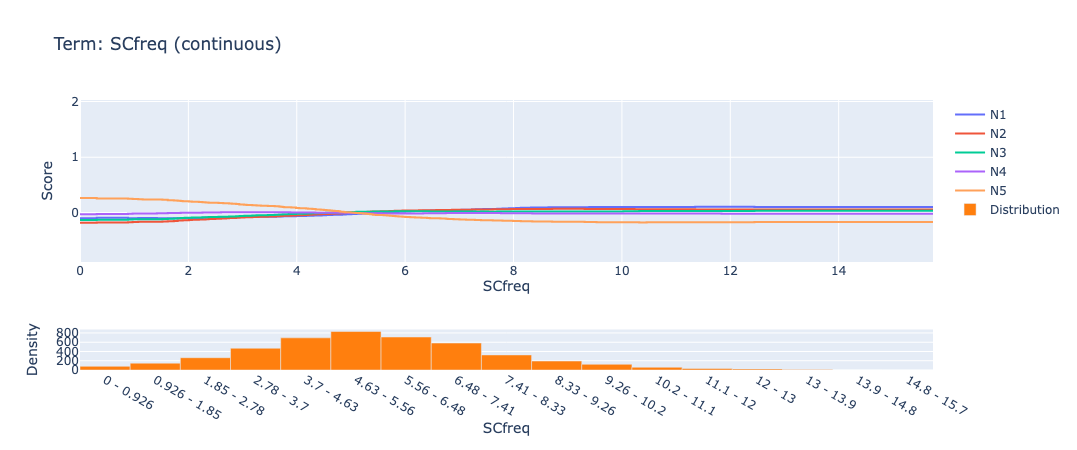
\includegraphics[scale=.4]{img/EBM/EBMSCfreq}
    \caption[Contribution of Subordinating Conjuction Frequency]{This chart represents how the feature of Suboardinating Conjunction frequency contributes to the prediction of each proficiency level}
    \label{fig:EBMSCfreq}
\end{figure}

Several morphological complexity indicators also appeared among the top features. Both MCI-5 surface and MCI-10
surface were ranked in the top ten, indicating that surface-level morhpological diversity increases with
proficiency. Additionaly, MCI-10 Inflection, a variant of the MCI measuring inflectional diversity, was also
influential. This is a surprising finding as due to the increased text window size leading to shorter texts being
 excluded. Although this was the only MCI measure that was found to distinguish between the N1 and native speaker
group, as discussed in the previous chapter, this feature also seemed to be used to differentiate the N1 proficiency
levels as seen in Figure~\ref{fig:EBMMCI10inflection}.

\begin{figure}[h!]
    \centering
    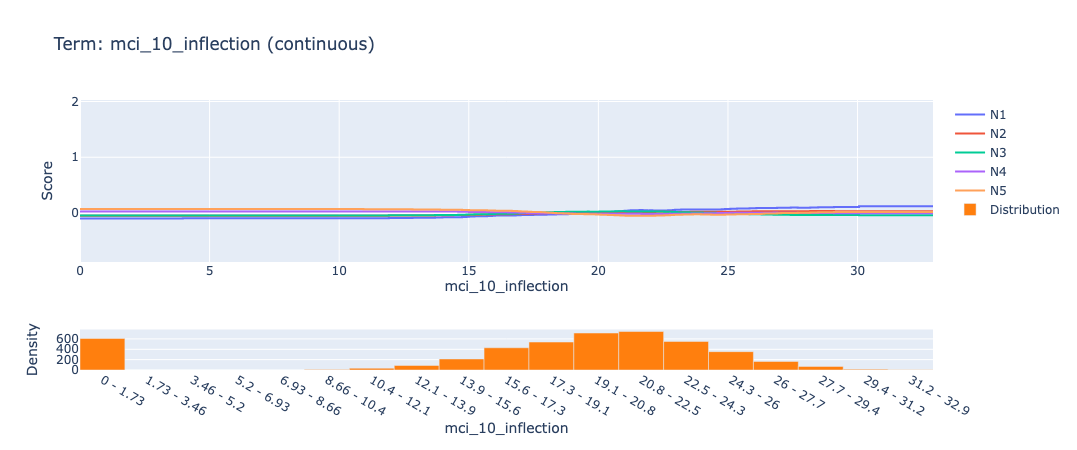
\includegraphics[scale=.4]{img/EBM/MCI10inflection}
    \caption[Contribution of MCI 10 Inflection measure]{This chart represents how the feature of MCI10 inflection measure contributes to the prediction of each proficiency level}
    \label{fig:EBMMCI10inflection}
\end{figure}

JRMA Function MATTR and JRMA All MATTR also ranked within the top 15 as morphological diversity measures. This
suggests that variation in function, and content morphemes, which can also reflect grammatical eleboration as a
relevant factor in distinguishing between proficiency levels. As can be seen in Figure~\ref{fig:JRMAallMATTR}, a higher
all_MATTR
score leads distinguishes between the advanced (N1 and N2) and beginner and intermediate proficiency levels.

\begin{figure}[h!]
    \centering
    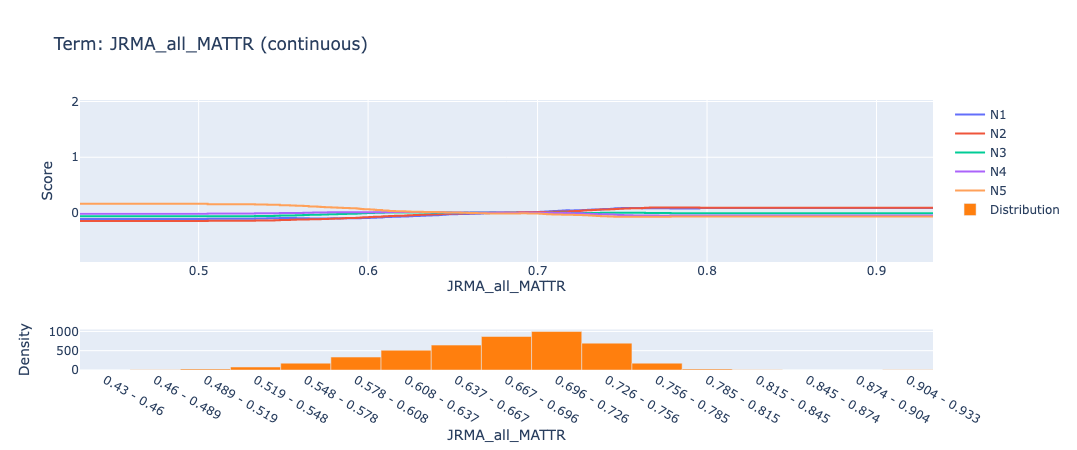
\includegraphics[scale=.4]{img/EBM/JRMAallMATTR}
    \caption[Contribution of JRMA function and content morphemes]{This chart represents how the feature of MATTR of content and function morphemes contributes to the prediction of each proficiency level}
    \label{fig:JRMAallMATTR}
\end{figure}


LFP OOV Percent (percentage of tokens outside the 10k frequency band)


Ukemi - passive form was the only criterial feature in top 15.


\section{Discussion}

% Make conrete citations
The results above provide partial support for developmental patterns identified in the previous chapters. In
particular, some features showed a clear trajectory of increased usage of complexity across levels, supporting
earlier corpus based findings and previous literature. However the predictive power of many features was moderate,
as found in the f1 scores, and some expected distinctions between adjacent levels (e.g. N3 vs N2) were not captured
effectively.

This suggests that while form-based measures of grammatical complexity and frequency based criterial features can be
useful, they may not be sufficienct in isolation. Some grammatical forms exhibit nuanced usage that depends on
semantic, pragmatic, or discourse-level factors which are not easily captured through surface-form
analysis alone.

The model's diminished performance, particularly for N2 and N1 as evidenced by lower f1-scores and the high number
of misclassifications in the confusion matrix (Figure~\ref{fig:conMA}), points to inherent challenges in
classifying these adjacent proficiency levels. The significant overlap observed in predictions (e.g. N3 misclassified
as N2 and N4) suggests that the linguistic differences between intermediate and advanced levels are subtler and less
discretely based on the current feature set. It is plausible after all, that learners at adjacent intermediate
levels exhibit similar linguistic characteristics than, for example, a beginner (N5) and an advanced learner (N1).
This continuous nature of language development makes sharp categorical distinctions difficult for any model.

The small sample size of N1 group (44 participants, 224 texts) significantly impacted its classification accuracy (
F1-score
of 0.17 in Table~\ref{tab:trainingResults}). With fewer examples, the model had limited data to learn the specific
criteria that distinguish N1 texts from other levels, leading to a high rate of misclassification, particularly into
N2 and N3 categories. This data imbalance likely constrained the model's ability to fully capture the
characteristics of advanced learners.


\subsection{Limitations and Difficulties}
The corpus, consisting of uncorrected learner language, posed challenges for feature extraction. Misspellings and
grammatical errors common in learner output could lead to incorrect tokenization and POS tagging by the underlying
NLP tools (e.g. SpaCy's Ginza package), thus impacting the accuracy of extracted features. For instance, irregular
forms of "mispellings" might be incorrectly counted as out-of-vocabulary words (in the context of the LFP complexity
measure), rather than as specific error types. More crucially, the morphological complexity of Japanese,
particularly with compound verbs and auxiliary constructions (e.g. 「言い切る」 as one verb vs. 「食べ切る」 parsed into two
parts), meant that rule-based feature extraction struggled with consistency. This could lead to undercounting or
miscategorizing certain complex forms, which are critical indicators of advanced proficiency.

The variability in text length, with some text being very short, likely affected the reliability of certain
density-based metrics, such as MTLD (Mean Type-Token Ratio), if it were included. Such metrics are sensitive to text
length, and calculation over very short texts can yield less stable or representative values, potentially
introducing noise into the feature set.

While features like coordinate clauses per sentence were highly important, the accuracy of their extraction was
dependent on the underlying tokenizer's ability to correctly identify conjunctions and clause boundaries. As noted
previously, many Japanese conjunctions can be used in both coordinating and subordinating contexts, and rule-based
parsers like SpacCy may not fully account for contextual nuances. This potential inaccuracy in the input features
could directly limit the model's ability to use these syntactic measures for precise classification. A more robust,
context-aware parsing system would likely improve the quality of these features.

The feature extractor largely focused on form-based grammatical constructs that are relatively easier to identify
programmatically and are common in standardized written Japanese. This approach may have overlooked more nuanced,
use-based grammatical patterns that could be highly discriminative of proficiency. Futhermore, the reliance on rules
for standardized written language means that variations due to dialects or highly casual written forms, if present
in the learner corpus, would not have been accurately captured, potentially missing valuable information for
classification.

A significant limitation of the current study was the exclusion of learner errors as a direct feature. Different
proficiency levels are often
characterized by distinct error patterns, as was illustrated in \citet{Hawkins_Buttery_2010}.  The
developmental tradjectory of errors, where specific error types and frequencies change systematically with
proficiency, could provide highly discriminative information for the model.
Incorporating
systematic error analysis as a
feature
set
could provide
highly discriminative information, potentially leading to substantial improvements in classification accuracy,
especially for distinguishing between adjacent intermediate and advanced levels where subtle error reductions or
shifts in error types might b proficiency levels used as the target classes. While these levels have been validated \citet{jcat_interpretation_guide}, they are primarily based on recognition tasks (reading and listening) and do not directly assess productive skills like writing or speaking. Therefore, the proficiency labels assigned to the learner texts, derived from J-Cat, are approximations of a broader construct of proficiencu. There can be considerable variance in the productive language capabilities of individuals who score similarly on the JLPT, which might introduce inherent 'noise' or ambiguity into the dataset, further complicating the task of classification for the model.

While EBM demonstrated capability to classify JLPT levels better than chance, performance highlights the inherent
complexity of distinguishing between closely related proficiency levels in a continuous developmental specture. The
identified features were significant, but future improvements would benefit from addressing the methodological
challenges in feature extraction, particularly for nuanced Japanese linguistic structures, and exploring the
integration of error-based features.